\section{Q-Band-Oriented Modeling}

\subsection{Reduced Roll-Sloshing Excitation Model}
Q-band ART does not require the online controller to predict the full liquid state. A reduced model is used only to explain which lateral-acceleration components are dangerous. The unsprung/base motion is represented by a lateral cart, the sprung tank body by a roll pendulum, and the dominant liquid mode by a pendulum attached to the tank body. Let
\begin{equation}
    \mathbf{x}_r=[\phi,\theta]^\T ,
\end{equation}
where $\phi$ is the tank-body roll angle and $\theta$ is the relative liquid sloshing angle. Around a nominal operating point, the coupled roll-sloshing dynamics can be written as
\begin{equation}
    \mathbf{M}\ddot{\mathbf{x}}_r+\mathbf{C}\dot{\mathbf{x}}_r+\mathbf{K}\mathbf{x}_r=\mathbf{B}_a \ay ,
    \label{eq:reduced_roll_slosh}
\end{equation}
where $\ay$ is the lateral acceleration generated by steering and tracking. The off-diagonal terms in $\mathbf{M}$ and $\mathbf{K}$ describe the coupling between suspension roll and liquid motion. Therefore, the dangerous frequency is not necessarily the isolated liquid natural frequency or the isolated roll frequency.

\begin{figure}[!t]
\centering
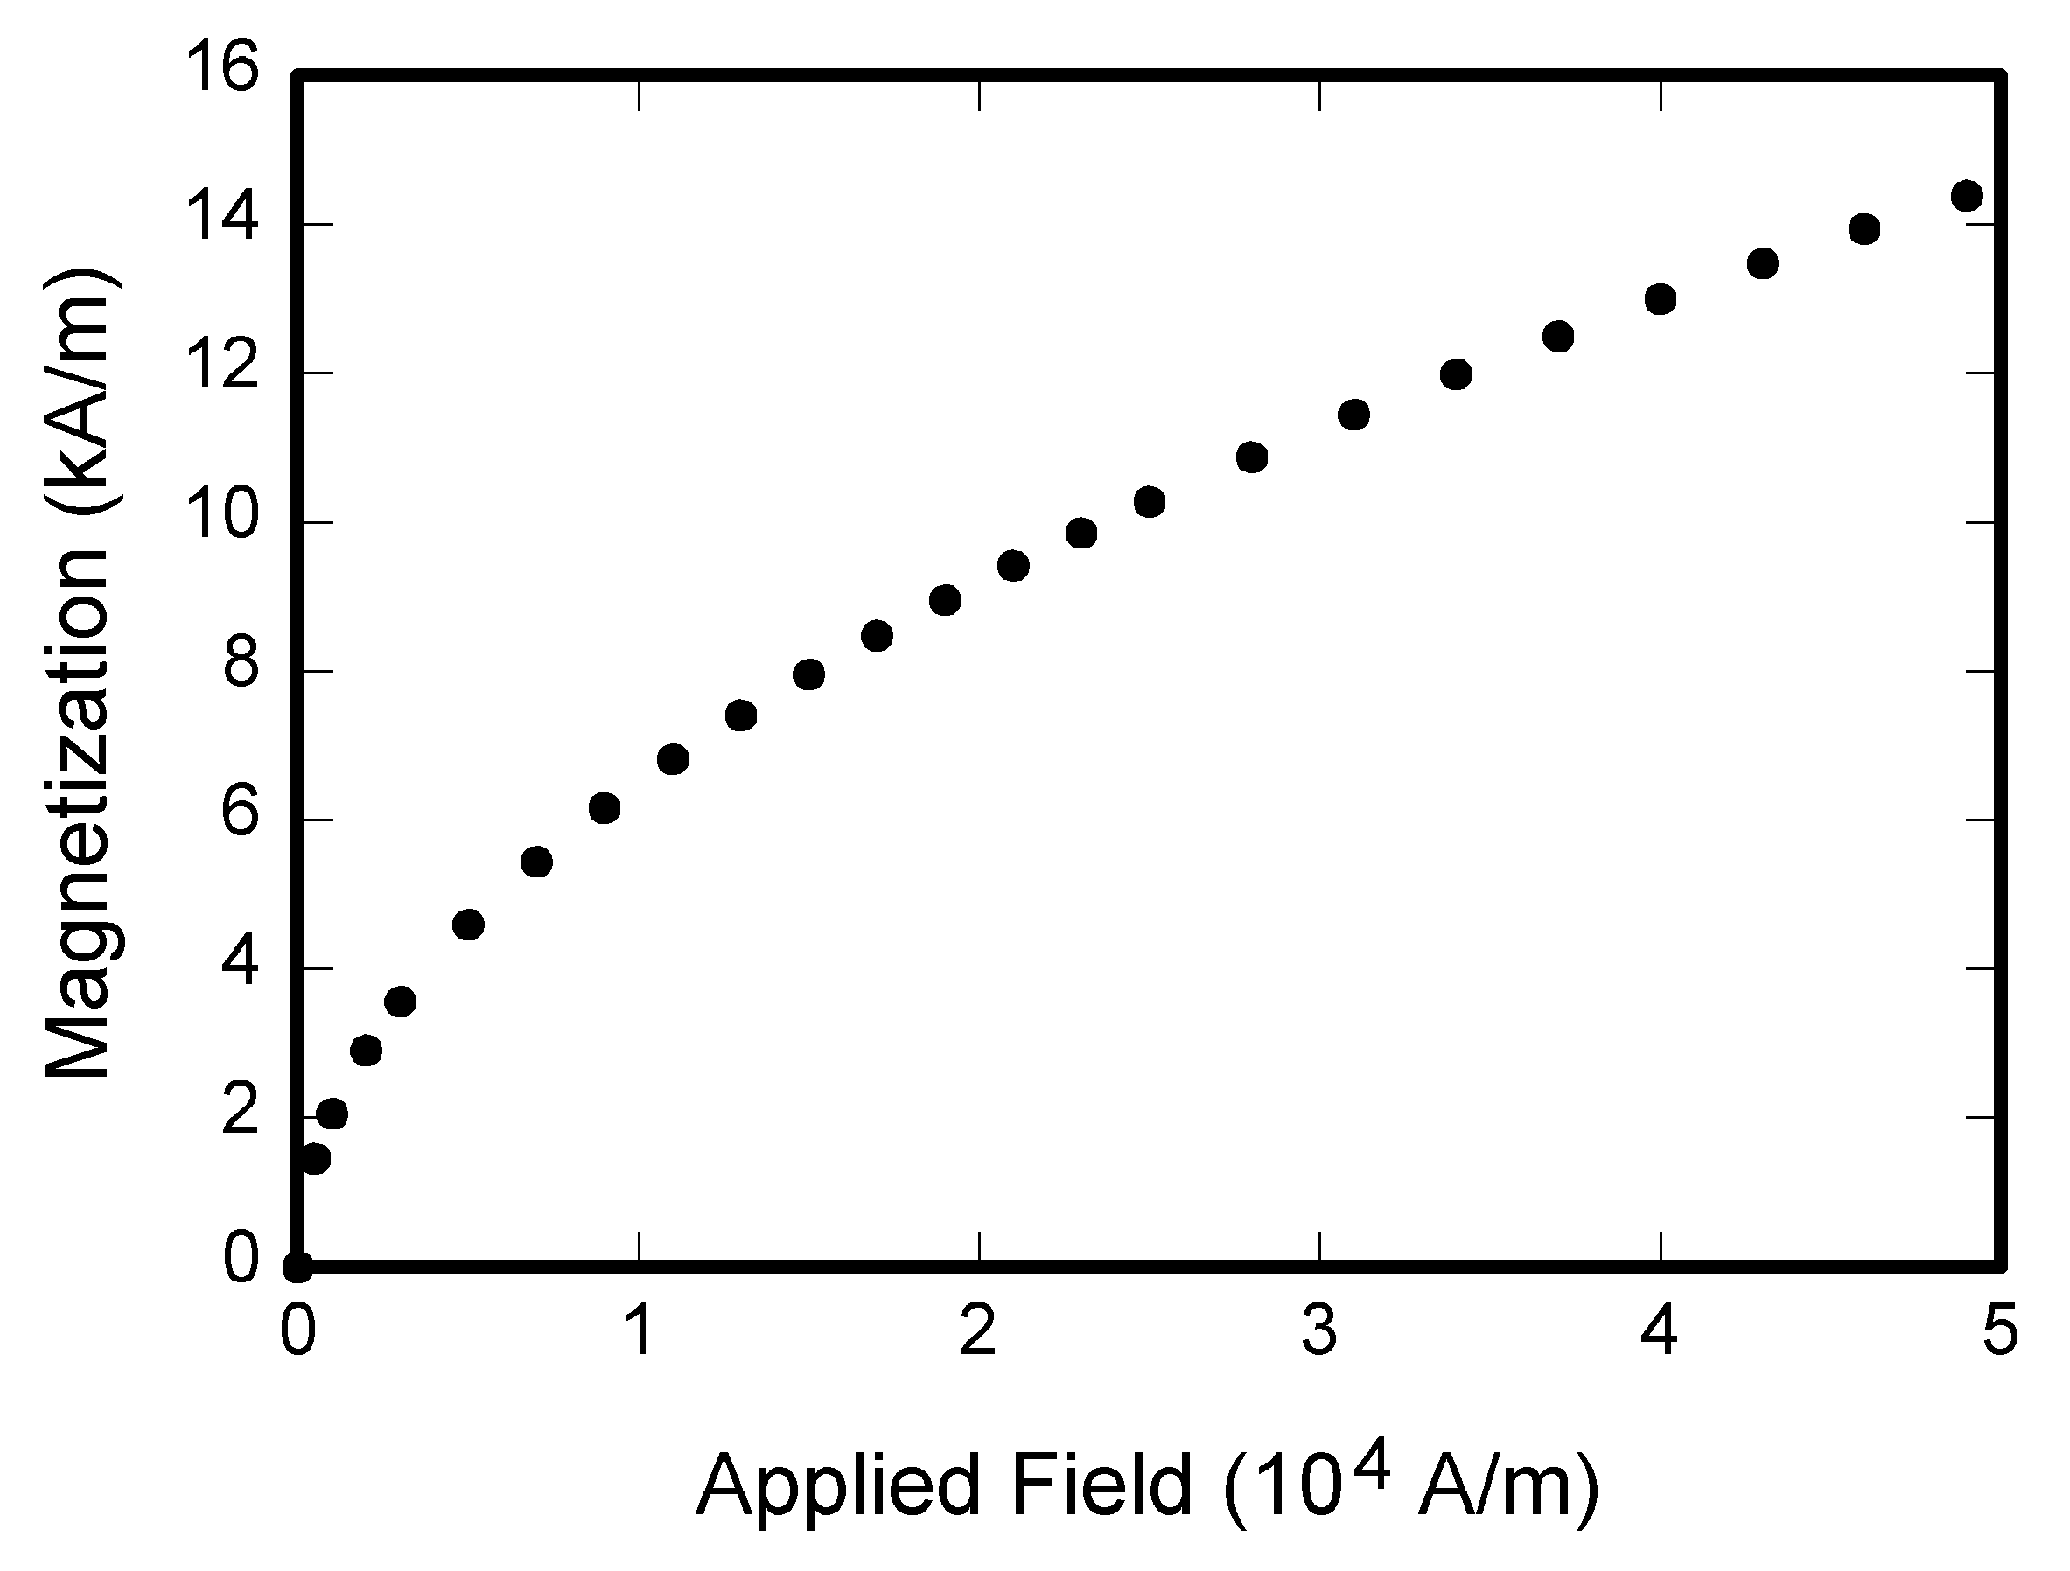
\includegraphics[width=\linewidth]{fig/fig1.png}
\caption{Reduced lateral model used to derive the Q-band concept. The online controller only needs the predicted lateral acceleration, while roll, sloshing, and LTR-related quantities are used for interpretation and validation.}
\label{fig:simplified_model}
\end{figure}
% TODO（作者）：将 fig1.png 替换为简化侧向模型图。建议左侧画半挂液罐车，右侧画小车-悬架倒立摆-液体正摆；标注 a_y、phi、theta、risk output。不要放太多参数，避免会议论文图太拥挤。

\subsection{Critical Band and Risk Bound}
Let the rollover-risk output be
\begin{equation}
    z=C_z\mathbf{x}_r+D_z\ay ,
\end{equation}
where $z$ can represent dynamic LTR, roll moment, roll-rate-weighted risk, or another calibrated rollover proxy. From \eqref{eq:reduced_roll_slosh}, the input-output frequency response is
\begin{equation}
    G_{za}(s)=C_z(s^2\mathbf{M}+s\mathbf{C}+\mathbf{K})^{-1}\mathbf{B}_a+D_z .
    \label{eq:freq_response}
\end{equation}
The Q-band $\mathcal{B}_i=[f_i^-,f_i^+]$ is selected around the peak or broad-peak region of $|G_{za}(j2\pi f)|$. In this work the main band is centered on the dominant sloshing-related response, with additional bands covering secondary and higher-frequency coupled excitations.

The following frequency-domain argument explains the safety meaning of Q-band suppression. If $|G_{za}(j2\pi f)|\leq \bar{G}_{\mathcal{B}}$ in a target band and the input component in that band has energy $\|a_{y,\mathcal{B}}\|_2^2$, then
\begin{equation}
    \|z_{\mathcal{B}}\|_2 \leq \bar{G}_{\mathcal{B}}\|a_{y,\mathcal{B}}\|_2 .
\end{equation}
Thus, limiting the band energy of $\ay$ gives a conservative bound on the risk output caused by that band. This is a sufficient safety explanation, not a replacement for full vehicle validation.

% TODO（作者）：最终稿需要给出由扫频、TruckSim 或模型车辨识得到的危险频带。当前 MATLAB 脚本采用 0.35--0.75 Hz 作为主频带，并覆盖 0.75--1.45 Hz 等次级频段；后续应写清楚这些频段的标定来源。

\subsection{Tracking Model and Disturbance Compensation}
For online tracking, the controller uses a low-dimensional prediction model that provides $\mathbf{A}_y$ over the horizon. In the engineering implementation, this prediction layer can be a kinematic or two-degree-of-freedom tractor model, while the validation object is the semi-trailer tank truck model in TruckSim and the model-truck platform. For the dynamic version,
\begin{equation}
\begin{aligned}
    \dot v_y &= \frac{F_{yf}\cos\delta+F_{yr}}{m_{\mathrm{eq}}}-v_xr+d_y,\\
    \dot r &= \frac{l_fF_{yf}\cos\delta-l_rF_{yr}}{I_{z,\mathrm{eq}}}+d_r,
\end{aligned}
\label{eq:tractor_2dof}
\end{equation}
where $d_y$ and $d_r$ collect trailer force, liquid sloshing, tire mismatch, and parameter error. An extended-state observer estimates the dominant residual, and a hitch-angle estimator schedules $m_{\mathrm{eq}}$ and $I_{z,\mathrm{eq}}$ as low-frequency articulated-vehicle priors. The remaining unmodeled dynamics are handled by safety margins and Q-band suppression rather than by adding liquid states to the optimizer.

\subsection{Online and Offline Quantities}
The online Q-band controller depends on predicted lateral acceleration, vehicle speed, steering state, yaw response, and reference preview. Liquid angle, true wheel loads, and high-fidelity LTR are not required online. They are used offline to calibrate the dangerous bands and to evaluate simulation or model-truck safety. This separation is important for trailer-sensing-limited deployment.
